%-----------------------------------------------------------------------------------------------------------------------------------------------%
%	The MIT License (MIT)
%
%	Copyright (c) 2021 Jitin Nair
%
%	Permission is hereby granted, free of charge, to any person obtaining a copy
%	of this software and associated documentation files (the "Software"), to deal
%	in the Software without restriction, including without limitation the rights
%	to use, copy, modify, merge, publish, distribute, sublicense, and/or sell
%	copies of the Software, and to permit persons to whom the Software is
%	furnished to do so, subject to the following conditions:
%	
%	THE SOFTWARE IS PROVIDED "AS IS", WITHOUT WARRANTY OF ANY KIND, EXPRESS OR
%	IMPLIED, INCLUDING BUT NOT LIMITED TO THE WARRANTIES OF MERCHANTABILITY,
%	FITNESS FOR A PARTICULAR PURPOSE AND NONINFRINGEMENT. IN NO EVENT SHALL THE
%	AUTHORS OR COPYRIGHT HOLDERS BE LIABLE FOR ANY CLAIM, DAMAGES OR OTHER
%	LIABILITY, WHETHER IN AN ACTION OF CONTRACT, TORT OR OTHERWISE, ARISING FROM,
%	OUT OF OR IN CONNECTION WITH THE SOFTWARE OR THE USE OR OTHER DEALINGS IN
%	THE SOFTWARE.
%	
%
%-----------------------------------------------------------------------------------------------------------------------------------------------%

%----------------------------------------------------------------------------------------
%	DOCUMENT DEFINITION
%----------------------------------------------------------------------------------------

% article class because we want to fully customize the page and not use a cv template
\documentclass[a4paper,12pt]{article}

%----------------------------------------------------------------------------------------
%	FONT
%----------------------------------------------------------------------------------------

% % fontspec allows you to use TTF/OTF fonts directly
% \usepackage{fontspec}
% \defaultfontfeatures{Ligatures=TeX}

% % modified for ShareLaTeX use
% \setmainfont[
% SmallCapsFont = Fontin-SmallCaps.otf,
% BoldFont = Fontin-Bold.otf,
% ItalicFont = Fontin-Italic.otf
% ]
% {Fontin.otf}

%----------------------------------------------------------------------------------------
%	PACKAGES
%----------------------------------------------------------------------------------------
\usepackage{url}
\usepackage{parskip} 	

%other packages for formatting
\RequirePackage{color}
\RequirePackage{graphicx}
\usepackage[usenames,dvipsnames]{xcolor}
\usepackage[scale=0.9]{geometry}

%tabularx environment
\usepackage{tabularx}

%for lists within experience section
\usepackage{enumitem}

% centered version of 'X' col. type
\newcolumntype{C}{>{\centering\arraybackslash}X} 

%to prevent spillover of tabular into next pages
\usepackage{supertabular}
\usepackage{tabularx}
\newlength{\fullcollw}
\setlength{\fullcollw}{0.47\textwidth}

%custom \section
\usepackage{titlesec}				
\usepackage{multicol}
\usepackage{multirow}

%CV Sections inspired by: 
%http://stefano.italians.nl/archives/26
\titleformat{\section}{\Large\scshape\raggedright}{}{0em}{}[\titlerule]
\titlespacing{\section}{0pt}{10pt}{10pt}

%for publications
\usepackage[style=authoryear,sorting=ynt, maxbibnames=2]{biblatex}

%Setup hyperref package, and colours for links
\usepackage[unicode, draft=false]{hyperref}
\definecolor{linkcolour}{rgb}{0,0.2,0.6}
\hypersetup{colorlinks,breaklinks,urlcolor=linkcolour,linkcolor=linkcolour}
\addbibresource{citations.bib}
\setlength\bibitemsep{1em}

%for social icons
\usepackage{fontawesome5}

%debug page outer frames
%\usepackage{showframe}

%----------------------------------------------------------------------------------------
%	BEGIN DOCUMENT
%----------------------------------------------------------------------------------------
\begin{document}

% non-numbered pages
\pagestyle{empty} 

%----------------------------------------------------------------------------------------
%	HEADING
%----------------------------------------------------------------------------------------

\begin{minipage}[c]{2.5cm}
    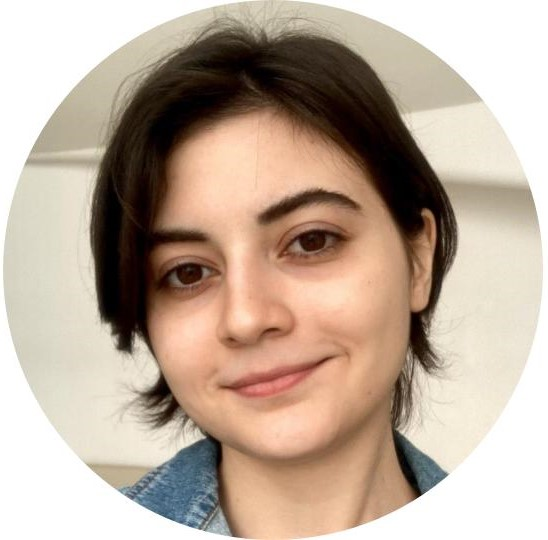
\includegraphics[width=2.5cm]{./avatar/avatar6.jpg}
\end{minipage}%
\hspace{1em}
\begin{minipage}[c]{\dimexpr\linewidth-2.5cm-15em\relax}
    \Huge{Arghavan Aslani}
\end{minipage}%
\begin{minipage}[c]{0.3\linewidth}
    \href{https://github.com/arghavanaslani}{\raisebox{-0.05\height}\faGithub\ github.com/arghavanaslani} \\ 
    \href{https://www.linkedin.com/in/arghavan-aslani/}{\raisebox{-0.05\height}\faLinkedin\ arghavan-aslani} \\ 
    \href{mailto:aslaniarghavan@gmail.com}{\raisebox{-0.05\height}\faEnvelope \ asaniarghavan@gmail.com} \\ 
    \href{tel:+989388687792}{\raisebox{-0.05\height}\faMobile \ +98.938.868.7792}
\end{minipage}

%----------------------------------------------------------------------------------------
%	EDUCATION
%----------------------------------------------------------------------------------------
\section{Education}
\begin{tabularx}{\linewidth}{@{}X r@{}}
    \textbf{B.Sc. in Electrical Engineering, University of Tehran, Tehran, Iran} & \textbf{2017 - 2022} \\
    \multicolumn{2}{@{}X@{}}{\emph{Control Major}} \\
\end{tabularx}

\begin{itemize}
    \item 
    \begin{tabularx}{\linewidth}{@{}X r@{}}
        Thesis: "LiveGaze: Real-Time Visualization of Multi-Source Eye-Tracking Data in an Integrated Application" & \href{https://github.com/arghavanaslani/livegaze}{Code Repository} \\
    \end{tabularx}
\end{itemize}


%----------------------------------------------------------------------------------------
% RESEARCH EXPERIENCE
%----------------------------------------------------------------------------------------

%Experience
\section{Research Experience}

\begin{tabularx}{\linewidth}{@{}X r@{}}
    \textbf{Crowd Cognition group, Ludwig Maximilians Universität München — Research Assistant} & \hfill Apr. 2022 - present \\[3.75pt]
    \href{https://crowdcognition.net/}{\raisebox{-0.05\height}\faGlobe\ crowdcognition.net} \\
\end{tabularx}

\begin{itemize}
    \item Exploratory Data Analysis - Collaboration with Museu do Amanhã, Rio de Janeiro, Brazil
    \begin{itemize}
        \item Developed a \href{https://crowd-cognition.github.io/Pupil-Invisible-Eye-Tracking-Data-Guide/}{comprehensive guide} for data collection with Pupil Invisible eye-tracking device, for the assistants, ensuring standardized procedures and high-quality data acquisition.
        \item Implemented and managed a labeling system for collected data, optimizing the organization and efficiency of subsequent analysis.
        \item Conducted in-depth data analysis, extracting meaningful insights and patterns, and delivered detailed reports to the museum, contributing valuable findings to the project's success.
    \end{itemize}
\end{itemize}

\begin{itemize}
    \item Investigating Variances in Visual Perception with Mobile Eye-Tracking
    \begin{itemize}
        \item Conducted a comprehensive data collection using the Pupil Invisible eye-tracking device in two conditions: individual and pair.
        \item Analyzed collected data using statistical tests to uncover insights in both spatial and temporal domains.
        \item Applied various similarity metrics to quantify spatial and temporal differences in the data.
        \end{itemize}
\end{itemize}

\begin{itemize}
    \item LiveGaze - Real-Time Visualization of Multi-Source Eye-Tracking Data
        \begin{itemize}
            \item Developed the Minimum Viable Product (MVP) in Flask framework, with ongoing development to enhance features and functionality.
            \end{itemize}
\end{itemize}
\vspace{\baselineskip} 

\begin{tabularx}{\linewidth}{@{}X r@{}}
    \textbf{ESLAB, University of Tehran — Lead Reseach Assistant} & \hfill July 2021 - August 2022 \\[3.75pt]
    \href{https://www.linkedin.com/company/eng-sci-lab/}{\raisebox{-0.05\height}\faLinkedin\ www.linkedin.com/company/eng-sci-lab} \\
\end{tabularx}

\begin{tabularx}{\linewidth}{@{}X r@{}}
    {- Developed a 2-DOF robot named "Spider-Paint" capable of translating images into drawings on a whiteboard using a marker.} & \hfill \href{https://github.com/arghavanaslani/spider-paint/blob/'spider-paint'/README.md}{Link to Videos} \\[3.75pt]
    {- Designed and implemented a control algorithm in C to operate two stepper motors on a vertical plane using a single Arduino.} & \hfill \href{https://github.com/arghavanaslani/spider-paint}{Link to Code} \\[3.75pt]
    {- Authored a paper accepted at the ISME Conference 2022 by consolidating contributions from various team members.}
\end{tabularx}
\vspace{\baselineskip} 
\vspace{\baselineskip} 


\begin{tabularx}{\linewidth}{@{}X r@{}}
    \textbf{CLIC, University of Tehran — Market Analyst} & \hfill July 2019 - Sep 2019 \\[3.75pt]
\end{tabularx}

\begin{tabularx}{\linewidth}{@{}X r@{}}
    {Conducted in-depth analysis to identify optimal markets for eye-tracking devices.} & \hfill \href{}{} \\[3.75pt]
    {Scheduled and facilitated meetings with potential customes.} & \hfill \href{}{} \\[3.75pt]
    {Prepared and delivered weekly progress reports on the analysis.} & \hfill \href{}{} \\[3.75pt]
\end{tabularx}

%----------------------------------------------------------------------------------------
%	PUBLICATIONS
%----------------------------------------------------------------------------------------

\section{Publications}

\begin{itemize}
    \item \textbf{Measuring Gaze Scan-Path Similarity Between Observers Using Mobile Eye-Tracking}\\
    Contributors: \textbf{A. Aslani}, D. Gulhan, A. Aliyeva, S. Saeedpour, O. Deroy, B. Bahrami\\
    Status: Under Preparation
\end{itemize}


\begin{itemize}
    \item \textbf{Design, Fabrication and Control of 2 DoF Robot in Vertical Plan}\\
    Authors: \textbf{A. Aslani}, E. Maani Miandob, H. Najafi, H. Bahreininan, M. Hemmati, M. Fakher\\
    Conference: The 30th Annual International Conference of the Iranian Society of Mechanical Engineers, 2022\\
    Publisher:  \href{https://civilica.com/doc/1468825/}{https://civilica.com/doc/1468825/}
\end{itemize}



%----------------------------------------------------------------------------------------
% WORK EXPERIENCE
%----------------------------------------------------------------------------------------

% \section{Work Experience}



%----------------------------------------------------------------------------------------
% EPROJECTS
%----------------------------------------------------------------------------------------

%Projects
% \section{Projects}

% \begin{tabularx}{\linewidth}{ @{}l r@{} }
% \textbf{Web Scraping for Job Advertisements in https://jobvision.ir} & \hfill \href{https://github.com/arghavanaslani/JobAdDB}{Link to Code} \\[3.75pt]
% \multicolumn{2}{@{}X@{}}{Developed in Python.
% Utilized BeautifulSoup, pandas, and requests for web scraping and data processing.
% Created a custom database due to the unavailability of existing datasets in the field.}  \\
% \end{tabularx}

%----------------------------------------------------------------------------------------
%	CERTIFICATIONS
%----------------------------------------------------------------------------------------

\section{Certifications}

\begin{tabularx}{\linewidth}{ @{}l r@{} }
    {Computational Neuroscience, Neuromatch Academy} & \hfill \href{https://portal.neuromatchacademy.org/certificate/ee23deef-9e73-4233-8c46-6e85375d9f1b}{Link to Certificate} \\[3.75pt]
    {Task-Orienred Course in Data Analysis with Python} & \hfill \href{https://quera.org/certificate/7p1aeaOn/}{Link to Certificate} \\[3.75pt]
    {Task-Orienred Course in SQL} & \hfill \href{https://quera.org/certificate/D4uYyhcQ/}{Link to Certificate} \\[3.75pt]
    \multicolumn{2}{@{}X@{}}{} 
\end{tabularx}

%----------------------------------------------------------------------------------------
%	VOLENTEER EXPERIENCE
%----------------------------------------------------------------------------------------
\section{Volenteer Experience}

\begin{itemize}
    \item 
    \begin{tabularx}{\linewidth}{@{}X r@{}}
        {Member of BTCS (Brain Tech and Cognitive Science Club)}\\
    \end{tabularx}
    \item 
    \begin{tabularx}{\linewidth}{@{}X r@{}}
        {Performer and Member of Council at Performing Arts Club} & \hfill \href{https://www.instagram.com/fanni_theater/}{Link to Instagram Page} \\[3.75pt]
    \end{tabularx}
\end{itemize}
%----------------------------------------------------------------------------------------
%	SKILLS
%----------------------------------------------------------------------------------------
\section{Technical Skills}
\begin{tabularx}{\linewidth}{@{}l X@{}}
    Data Analysis &  \normalsize{Python (Numpy, Pandas, Matplotlib, scikit-learn), SQL (Postgres, MySQL), MATLAB, R}\\
    Web Development &  \normalsize{Python (Flask, Django), HTML5, CSS, JavaScript}\\
    Operating Systems &  \normalsize{Linux(Ubuntu), Windows}\\  
    Tools &  \normalsize{Git, Jupyter Notebook, LATEX, Microsoft Office}\\ 
    
\end{tabularx}

%----------------------------------------------------------------------------------------
%	LANGUAGES
%----------------------------------------------------------------------------------------
% \section{Languages}
% \begin{tabularx}{\linewidth}{@{}l X@{}}
%     English &  \normalsize{Full Professional Proficiency(IELTS overall:7.5, L:8.5, R:7.5, W:7, S:7.5)}\\
%     Farsi(Persian) &  \normalsize{Native or bilingual proficiency}\\
%     % Turkish &  \normalsize{Limited working proficiency}\\  
%     % Arabic &  \normalsize{Elementary proficiency}\\ 
    
% \end{tabularx}

%----------------------------------------------------------------------------------------
%	REFERENCES
%----------------------------------------------------------------------------------------

\section{References}

\begin{itemize}
    \item \textbf{Dr. Bahador Bahrami} - \href{mailto:bahador.bahrami@psy.lmu.de}{bahador.bahrami@psy.lmu.de}\\
    Senior Research Scientist, Faculty of Psychology and Educational Sciences, Ludwig Maximilian University, Munich
    
    \item \textbf{Dr. Ehsan Maani Miandoab} - \href{mailto:e.maani@ut.ac.ir}{e.maani@ut.ac.ir}\\
    Assistant Professor, Faculty of Engineering Sciences, College of Engineering, University of Tehran, Iran
    
    \item \textbf{Prof. Ophelia Deroy} - \href{mailto:Ophelia.Deroy@lrz.uni-muenchen.de}{Ophelia.Deroy@lrz.uni-muenchen.de}\\
    Chair for Philosophy of Mind and Neuroscience, Ludwig Maximilian University, Munich
\end{itemize}


\end{document}
